\documentclass[aspectratio=169, 10pt]{beamer}

\usepackage[utf8]{inputenc}
\usepackage[T1]{fontenc}
\usepackage[brazil]{babel}
\usepackage{amsmath, amsfonts, amssymb}
\usepackage{graphicx}
\usepackage{booktabs}
\usepackage{xcolor}

% Tema e Cores Acadêmicas UFC
\usetheme{Madrid}
\usecolortheme{whale}
\definecolor{ufcblue}{RGB}{15, 44, 89}
\definecolor{ufcaccent}{RGB}{2, 132, 199}
\setbeamercolor{palette primary}{bg=ufcblue, fg=white}
\setbeamercolor{palette secondary}{bg=ufcaccent, fg=white}
\setbeamercolor{structure}{fg=ufcblue}
\setbeamercolor{block title}{bg=ufcblue, fg=white}
\setbeamercolor{block body}{bg=ufcblue!6, fg=black}
\setbeamertemplate{navigation symbols}{}

\title[Efeito Fotoelétrico — Tema 2]{Efeito Fotoelétrico por meio de Simulação Computacional}
\subtitle{TI0060 — Materiais Eletrônicos e Optoeletrônicos (1ª Avaliação)}
\author[Logan e Samuel Farias]{\textbf{Equipe (Tema 2):} Logan e Samuel Farias \\ \vspace{0.15cm} {\small Prof. Dr. Joacir Andrade}}
\institute[UFC]{Universidade Federal do Ceará (UFC) \\ Engenharia de Telecomunicações — 2026.2}
\date{Outubro de 2026}

\begin{document}

% =============================================================================
% SLIDE 1: O PROBLEMA: COMPORTAMENTO DA EMISSÃO FOTOELÉTRICA
% =============================================================================
\begin{frame}{1. O Problema: Comportamento da Emissão Fotoelétrica}
  \vspace{-0.15cm}
  \begin{block}{Tema 2 — Equipe: Logan e Samuel Farias (TI0060 - Prof. Joacir Andrade)}
    \textbf{Questão Central:} Como a frequência ($f$) e a intensidade ($I$) da radiação governam a emissão de elétrons de uma superfície metálica, e como podemos modelar e verificar esse comportamento computacionalmente?
  \end{block}

  \vspace{0.1cm}
  \begin{columns}[T]
    \begin{column}{0.48\textwidth}
      \begin{alertblock}{O Desafio Físico a Explicar}
        \footnotesize
        \begin{itemize}
          \item \textbf{Frequência de Corte Estrita ($f_0$):} Abaixo de $f_0$, nenhum elétron é liberado do metal, por maior que seja a intensidade luminosa.
          \item \textbf{Independência de $K_{\max}$ frente a $I$:} Aumentar a intensidade aumenta a quantidade de elétrons, mas não altera a energia máxima individual ($K_{\max}$).
          \item \textbf{Resposta Instantânea:} Emissão em $\sim 10^{-9}\text{ s}$, sem atraso de acúmulo contínuo de energia.
        \end{itemize}
      \end{alertblock}
    \end{column}

    \begin{column}{0.48\textwidth}
      \begin{exampleblock}{Parâmetros e Variáveis do Estudo}
        \footnotesize
        \begin{itemize}
          \item \textbf{Radiação Incidente:} Frequência ($f$), comprimento de onda ($\lambda$) e intensidade luminosa ($I$).
          \item \textbf{Cátodo Emissor:} Função trabalho ($\phi$) dos 9 metais da Aula 03 (do $\text{Na}$ com $2{,}28\text{ eV}$ à $\text{Pt}$ com $6{,}35\text{ eV}$).
          \item \textbf{Circuito Elétrico:} Potencial de frenagem ($-V_0$) e fotocorrente ($I_{\text{foto}}$).
        \end{itemize}
      \end{exampleblock}
    \end{column}
  \end{columns}
\end{frame}

% =============================================================================
% SLIDE 2: COMO RESOLVEMOS: MODELAGEM TEÓRICA E COMPUTACIONAL (LAYOUT LIMPO)
% =============================================================================
\begin{frame}{2. Como Resolvemos: Modelagem Teórica e Computacional}
  \vspace{-0.35cm}
  \begin{columns}[T]
    \begin{column}{0.48\textwidth}
      \small
      \textbf{1. Fóton e Barreira do Material ($\phi$):}
      \footnotesize
      \begin{itemize}
        \item Energia do Fóton: $E_f = h f = \frac{hc}{\lambda}$ \quad ($h \approx 4{,}136\times 10^{-15}\text{ eV}\cdot\text{s}$)
        \item Frequência de Corte: $f_0 = \frac{\phi}{h} \iff \lambda_0 = \frac{hc}{\phi}$
      \end{itemize}
    \end{column}

    \begin{column}{0.48\textwidth}
      \small
      \textbf{2. Balanço de Einstein e Frenagem ($V_0$):}
      \footnotesize
      \begin{itemize}
        \item Balanço Energético: $K_{\max} = hf - \phi = \frac{1}{2}m_e v_{\max}^2$
        \item Potencial de Frenagem: $q V_0 = K_{\max} \implies V_0 = \frac{h}{q}f - \frac{\phi}{q}$
      \end{itemize}
    \end{column}
  \end{columns}

  \vspace{0.10cm}
  \centering
  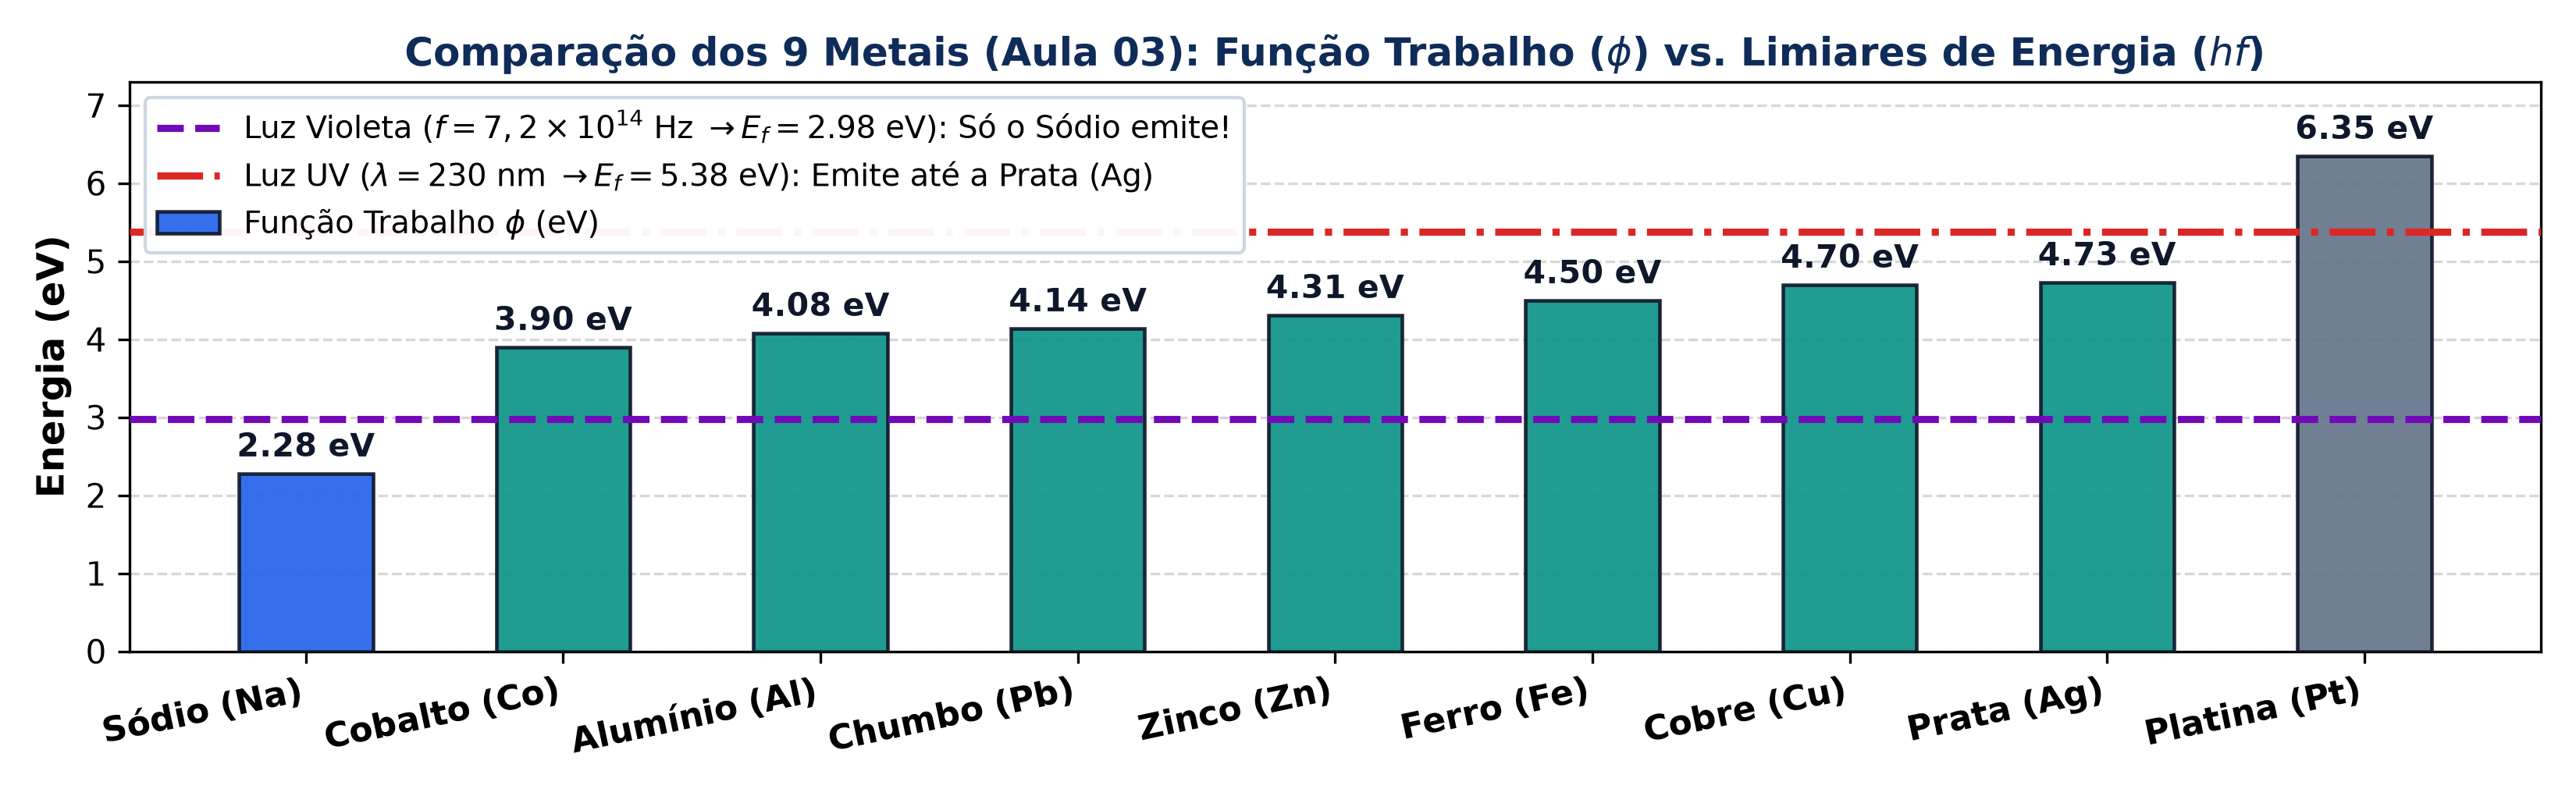
\includegraphics[height=3.60cm, width=0.88\textwidth, keepaspectratio]{fig3_comparacao_metais_barreira.png}
\end{frame}

% =============================================================================
% SLIDE 3: RESULTADOS 1 — INFLUÊNCIA DA FREQUÊNCIA E CASO DO SÓDIO
% =============================================================================
\begin{frame}{3. Resultados 1: Influência da Frequência e Estudo de Caso do Sódio}
  \begin{columns}[c]
    \begin{column}{0.57\textwidth}
      \centering
      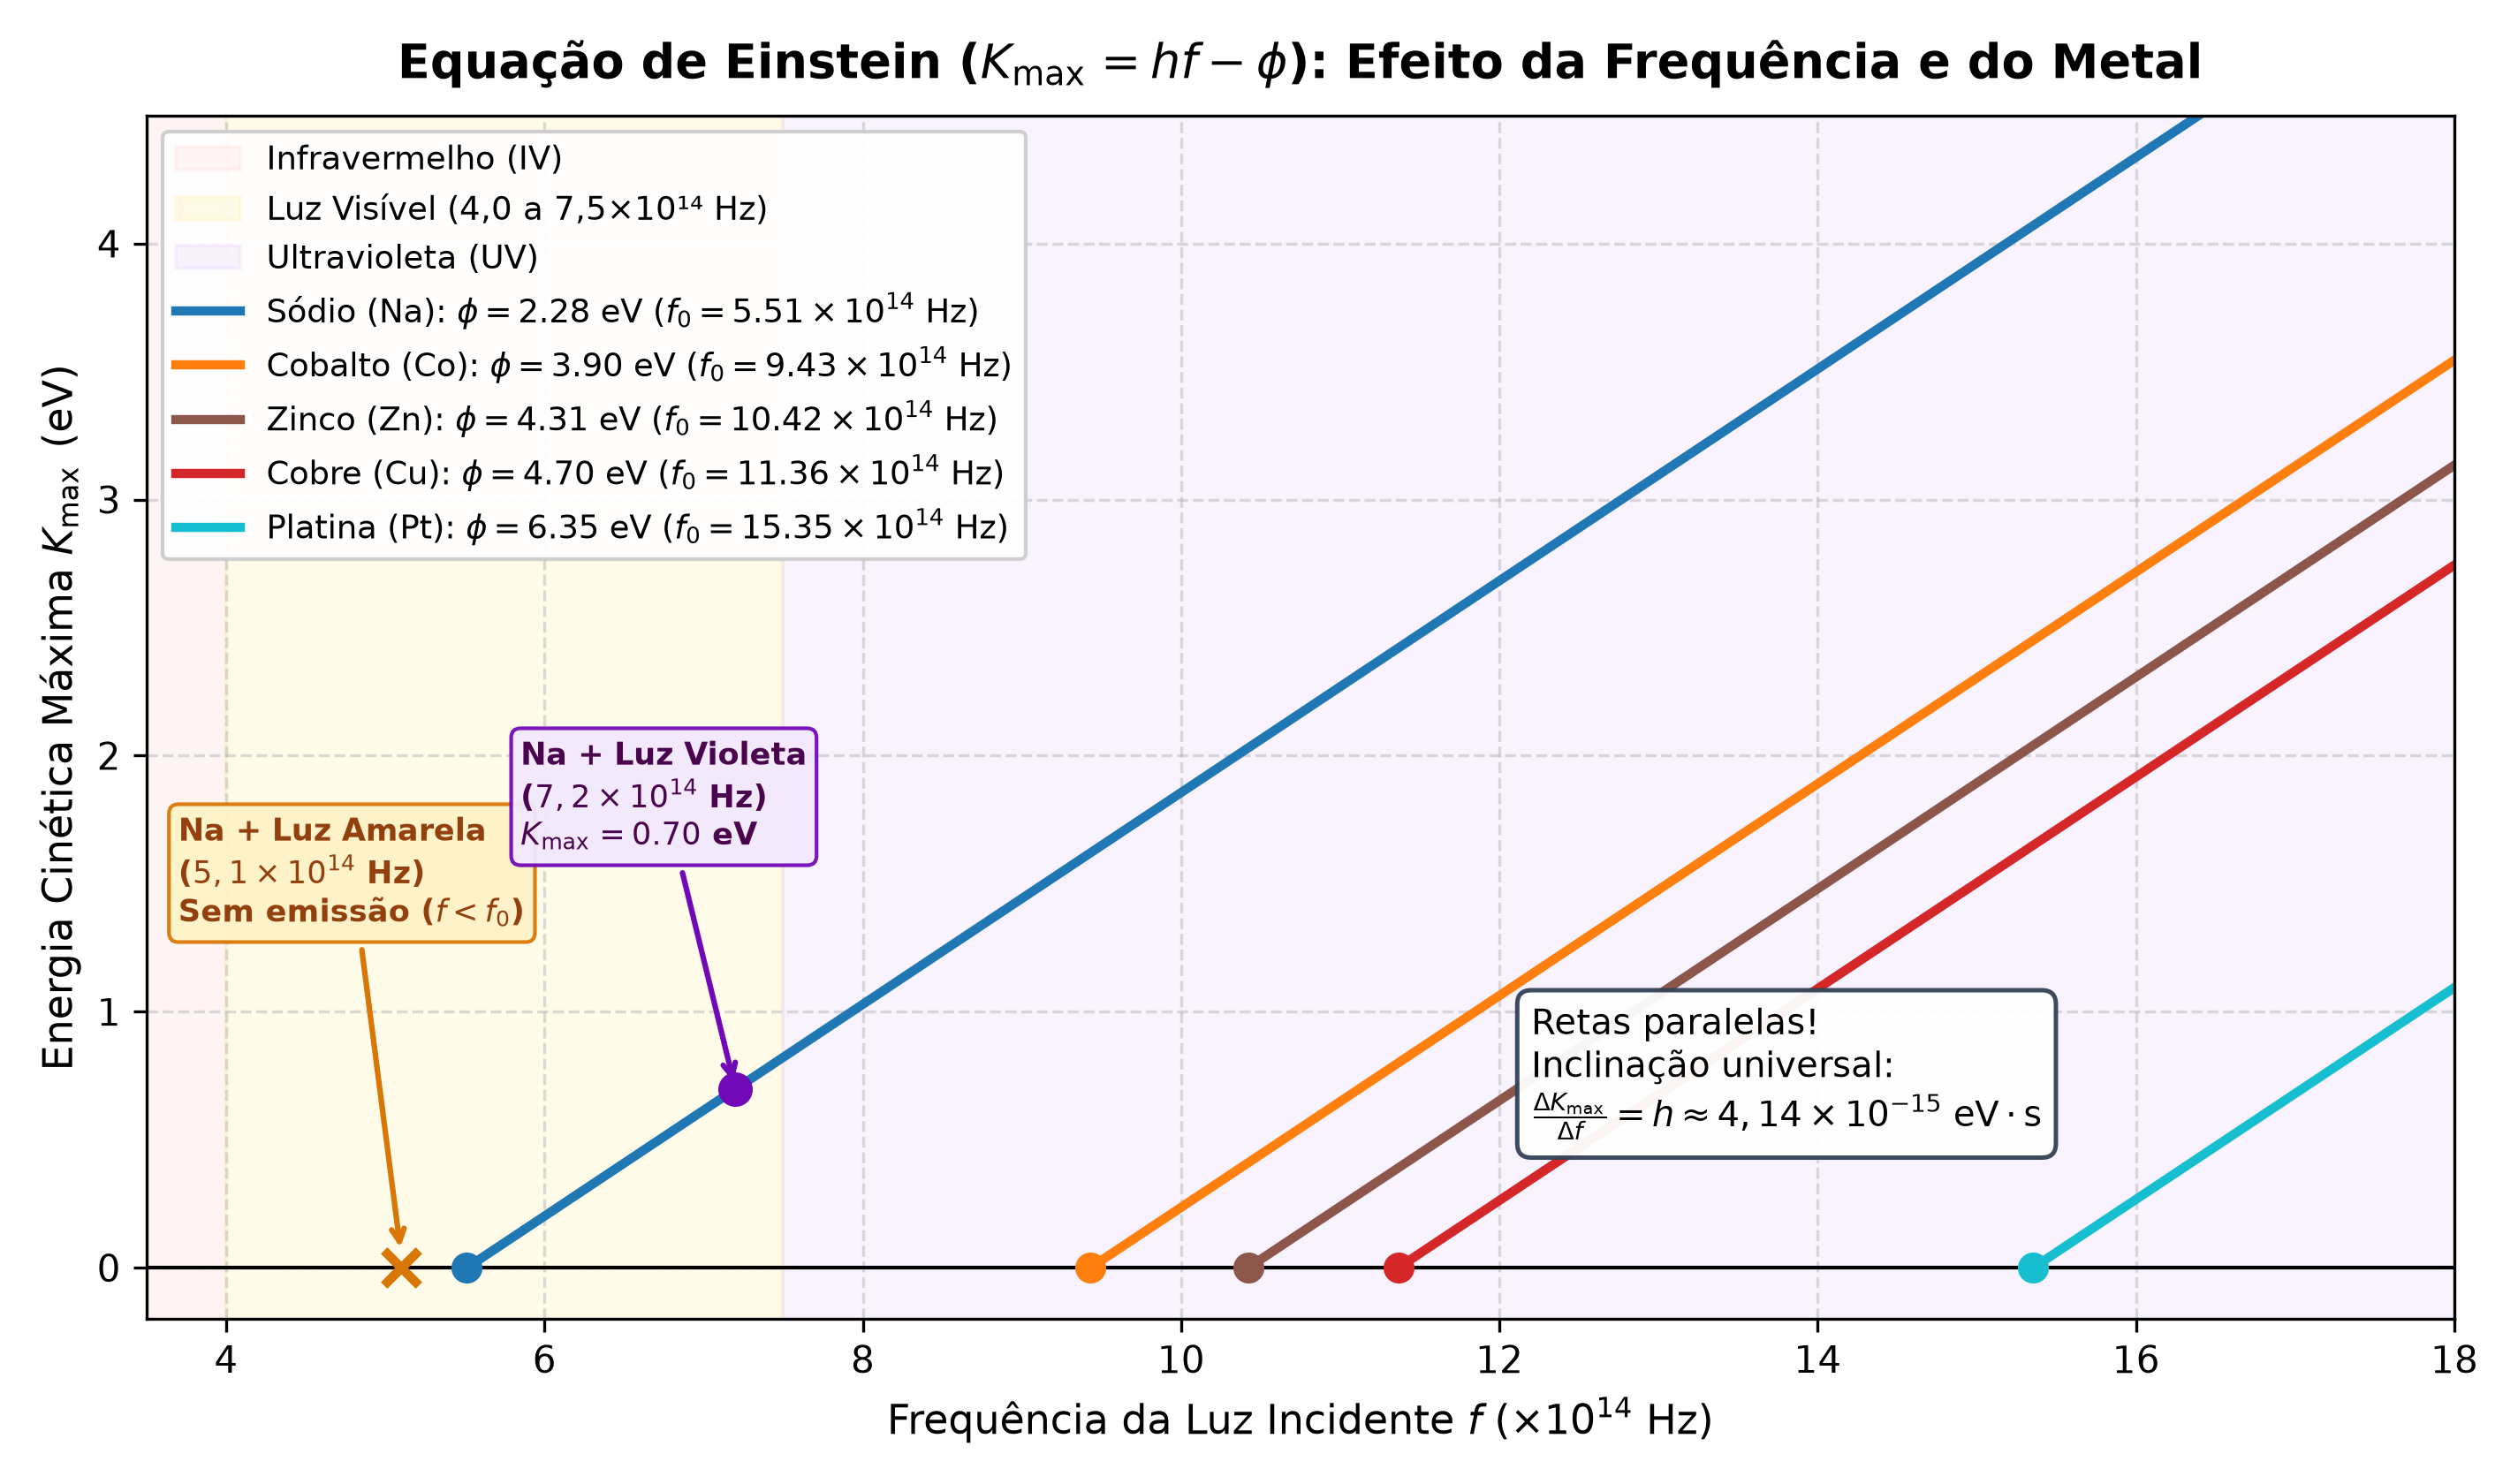
\includegraphics[width=\textwidth]{fig1_kmax_vs_frequencia.png}
    \end{column}

    \begin{column}{0.41\textwidth}
      \scriptsize
      \textbf{Estudo de Caso (Aula 03 — Sódio, $\phi = 2{,}28\text{ eV}$):}
      \vspace{0.1cm}
      \begin{table}
        \centering
        \begin{tabular}{lccc}
          \toprule
          \textbf{Cor ($f$)} & $E_f$ & $K_{\max}$ & \textbf{Emissão?} \\
          \midrule
          Vermelha ($4{,}3$) & $1{,}78\text{ eV}$ & $0{,}00\text{ eV}$ & Não \\
          Amarela ($5{,}1$)  & $2{,}11\text{ eV}$ & $0{,}00\text{ eV}$ & Não \\
          Verde ($5{,}6$)    & $2{,}32\text{ eV}$ & $0{,}04\text{ eV}$ & Sim \\
          Azul ($6{,}3$)     & $2{,}61\text{ eV}$ & $0{,}33\text{ eV}$ & Sim \\
          Violeta ($7{,}2$)  & $2{,}98\text{ eV}$ & $0{,}70\text{ eV}$ & Sim \\
          UV 300nm ($10{,}0$)& $4{,}13\text{ eV}$ & $1{,}85\text{ eV}$ & Sim \\
          \bottomrule
        \end{tabular}
      \end{table}
      \vspace{0.05cm}
      \begin{itemize}
        \item No Sódio ($f_0 = 5{,}51\times 10^{14}\text{ Hz}$), a luz \textbf{violeta} ejeta elétrons com $v_{\max} = 4{,}95\times 10^5\text{ m/s}$, enquanto a \textbf{amarela} não ejeta nada.
        \item Todas as retas têm a \textbf{mesma inclinação universal $h$}.
      \end{itemize}
    \end{column}
  \end{columns}
\end{frame}

% =============================================================================
% SLIDE 4: RESULTADOS 2 — INTENSIDADE vs. FREQUÊNCIA NA FOTOCORRENTE
% =============================================================================
\begin{frame}{4. Resultados 2: Intensidade ($I$) vs. Frequência ($f$) na Fotocorrente}
  \centering
  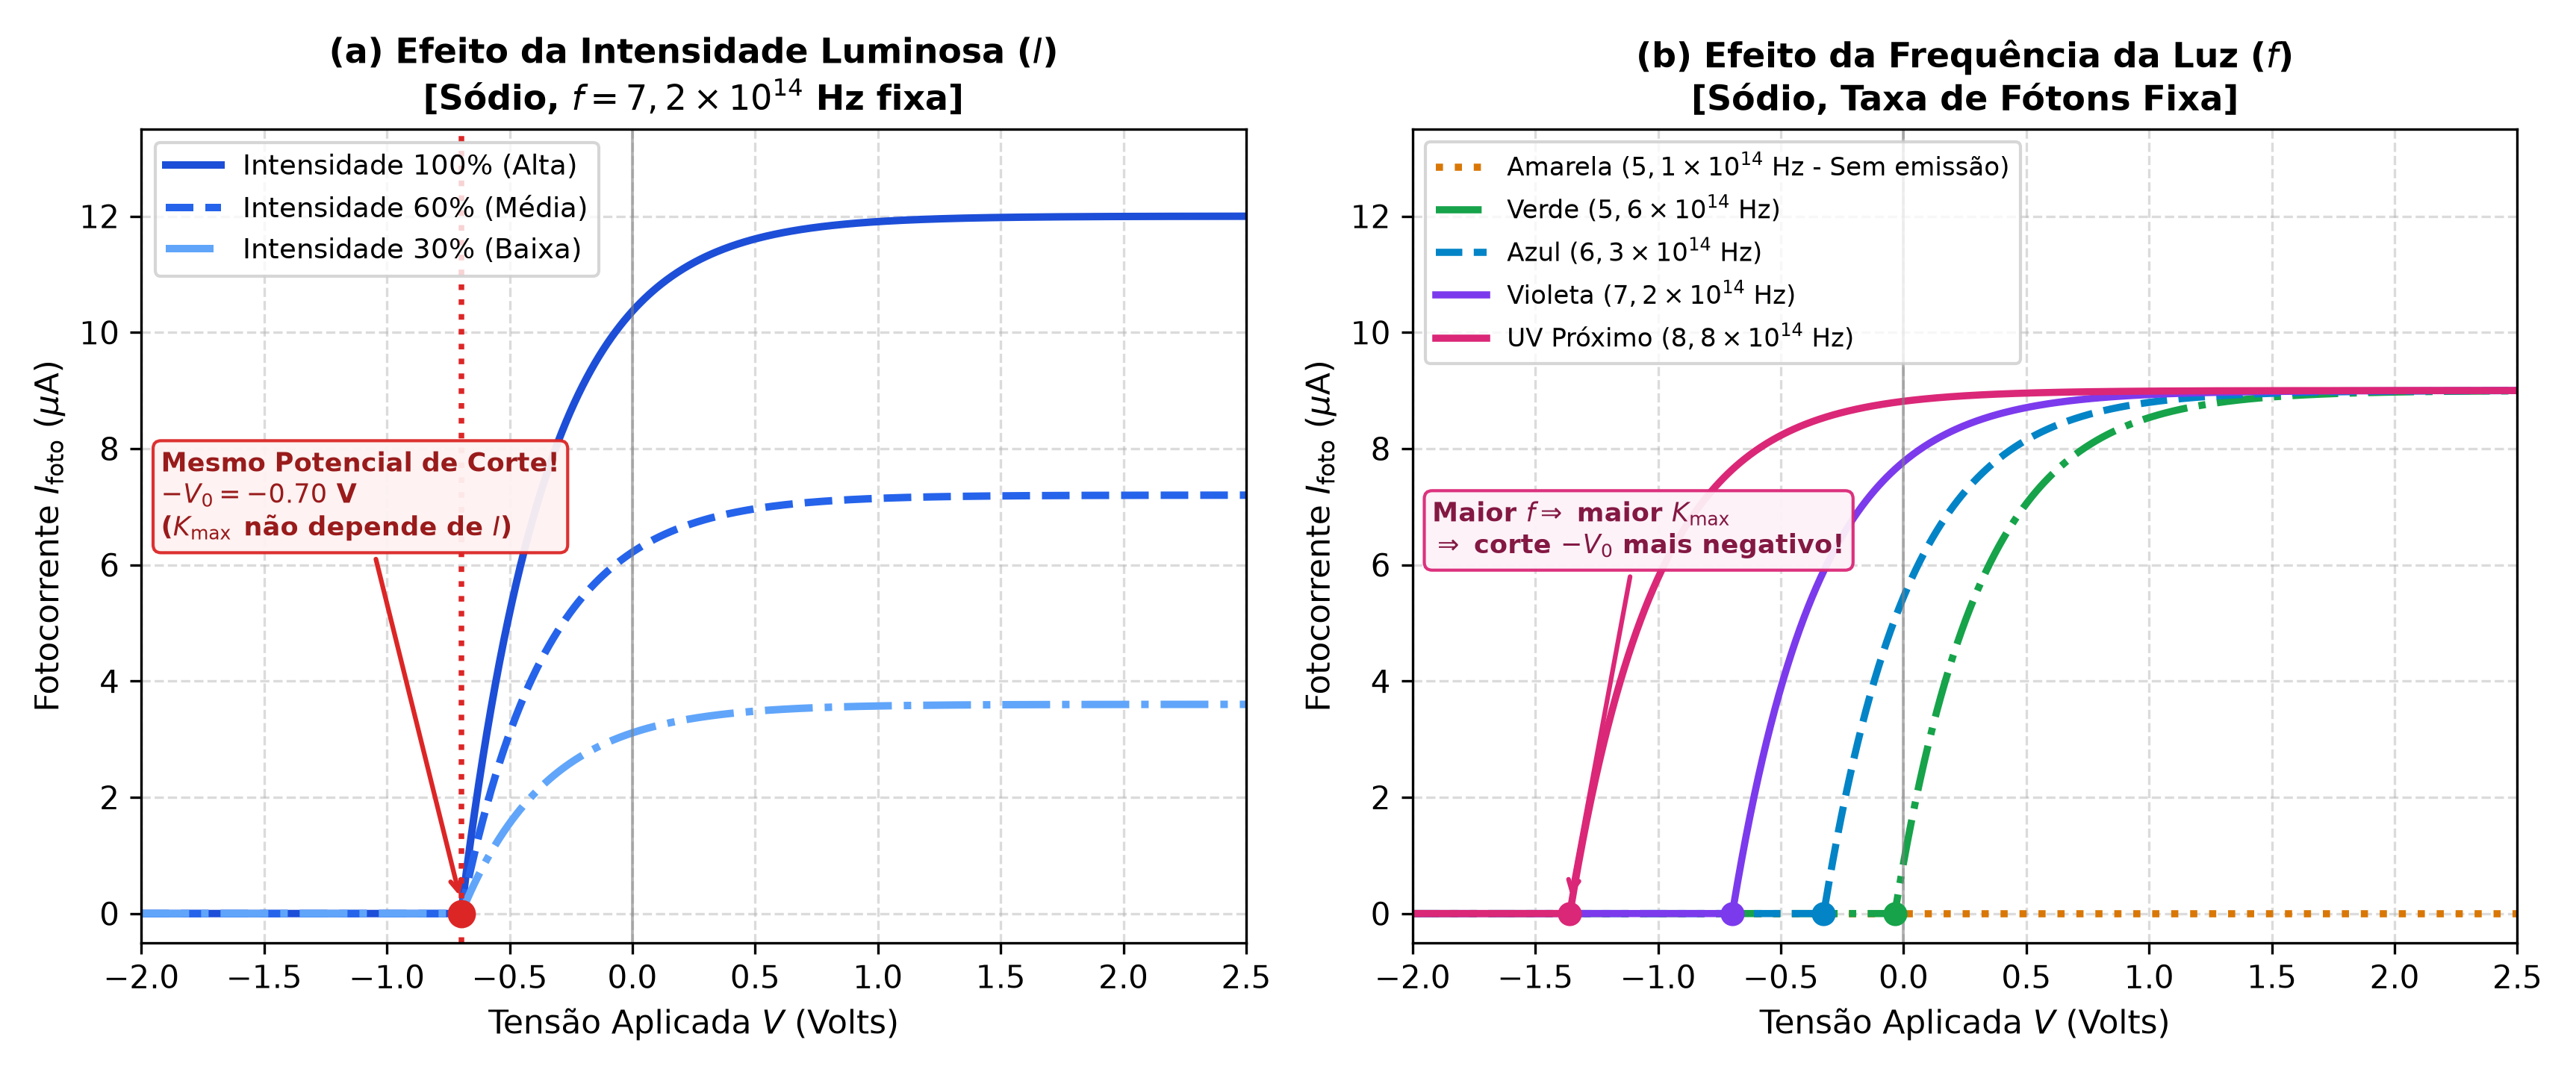
\includegraphics[width=0.92\textwidth]{fig2_corrente_vs_tensao.png}
  \vspace{-0.15cm}
  \begin{columns}[T]
    \begin{column}{0.48\textwidth}
      \scriptsize
      \textbf{(a) Variação da Intensidade ($f$ fixa):} Aumentar $I$ multiplica o número de fótons/s $\Rightarrow$ a fotocorrente de saturação cresce proporcionalmente, mas o potencial de corte $-V_0 = -0{,}70\text{ V}$ (e $K_{\max}$) \textbf{permanece estritamente fixo}.
    \end{column}
    \begin{column}{0.48\textwidth}
      \scriptsize
      \textbf{(b) Variação da Frequência (Taxa de fótons fixa):} Aumentar $f$ eleva a energia individual de cada fóton ($hf$) $\Rightarrow$ $K_{\max}$ cresce e o potencial de corte $-V_0$ torna-se progressivamente mais negativo.
    \end{column}
  \end{columns}
\end{frame}

% =============================================================================
% SLIDE 5: A SIMULAÇÃO: DEMONSTRAÇÃO INTERATIVA E CONCLUSÕES
% =============================================================================
\begin{frame}{5. A Simulação: Demonstração Interativa e Conclusões}
  \begin{columns}[T]
    \begin{column}{0.48\textwidth}
      \begin{block}{Simulador Interativo (HTML5 / Canvas)}
        \footnotesize
        \begin{itemize}
          \item Tubo a vácuo com fotocátodo e ânodo com visualização contínua dos fotoelétrons em tempo real.
          \item Seletor rápido dos 9 metais da Aula 03.
          \item Controles de espectro luminoso, intensidade e tensão coletor-cátodo.
          \item Botão de frenagem: aplica $-V_0$ e interrompe o fluxo de fotoelétrons na hora.
        \end{itemize}
      \end{block}
    \end{column}

    \begin{column}{0.48\textwidth}
      \begin{exampleblock}{Resposta ao Problema e Engenharia}
        \footnotesize
        \begin{itemize}
          \item \textbf{Frequência ($f$):} Qualidade energética ($hf$). Governa SE há ejeção, o valor de $K_{\max}$ e de $-V_0$.
          \item \textbf{Intensidade ($I$):} Quantidade de fótons/s. Modula a fotocorrente de saturação ($I_{\text{sat}}$).
          \item Aplicações vitais em fotodetectores PIN/APD de telecomunicações e espectroscopia óptica.
        \end{itemize}
      \end{exampleblock}
    \end{column}
  \end{columns}
\end{frame}

\end{document}
